\section{Raft}

На протяжении длительного времени для достижения консенсуса применялся алгоритм
Паксос, однако в кругах разработчиков распределённых систем он считался
чрезмерно сложным. В 2013 году был предложен новый подход под названием Raft,
ориентированный на упрощение понимания и реализации \cite{ongario14}.

В Raft каждый узел хранит локально журнал команд, исполняемых конечным автоматом.
Так как все процессы получают одинаковые входные данные и применяют идентичные
команды в одном и том же порядке, их конечные автоматы приходят к одинаковому
состоянию. Одно из отличий Raft заключается в том, что роль лидера здесь
вынесена на первый план: он координирует репликацию и манипуляции над конечным
автоматом. С этой точки зрения Raft схож с Мульти-Паксосом и атомарной рассылкой:
среди узлов выбирается лидер, который принимает решения и задаёт упорядочение
сообщений.

Алгоритм Raft определяет три основные роли:

\begin{itemize}
    \item Кандидат (candidate): Узел, который пытается стать лидером. Он набирает
        голоса большинства узлов. Если выборы не приводят к явному победителю,
        запускается новый период и процесс голосования повторяется.
    \item Лидер (leader): Временный управляющий кластером, обрабатывающий запросы
        клиентов и взаимодействующий с реплицируемым конечным автоматом. Лидер
        выбирается на определённый период, который идентифицируется возрастающим
        номером. Если лидер перестаёт отвечать или подозревается в отказе,
        начинается процедура переизбрания.
    \item Последователь (follower): Пассивный участник, хранящий записи журнала
        и реагирующий на запросы от лидера и кандидатов. По сути, в Raft он
        объединяет в себе функции акцептора и ученика из Паксоса. Каждый узел
        стартует в роли последователя.
\end{itemize}

Чтобы добиться упорядочения без жёсткой синхронизации часов, в Raft используются
периоды (эпохи, термы), в течение которых существует только один лидер. Каждый
период имеет уникальный номер, а команды внутри периода получают дополнительный
индекс. Узлы могут по-разному воспринимать текущий период (например, если они
пропустили этап выборов), но каждая отправляемая команда указывает номер
периода \cite{ongario14}. Если узел видит период с более высоким номером, он
обновляет своё значение периода.

Процесс выбора лидера инициируется, когда последователь не получает подтверждений
от текущего лидера, полагая, что тот вышел из строя. В этом случае последователь
переходит в состояние кандидата и собирает голоса большинства узлов, стремясь
стать новым лидером.

На рис. \ref{fig:raft} приведена схема раунда Raft.

\begin{figure}
  \centering
  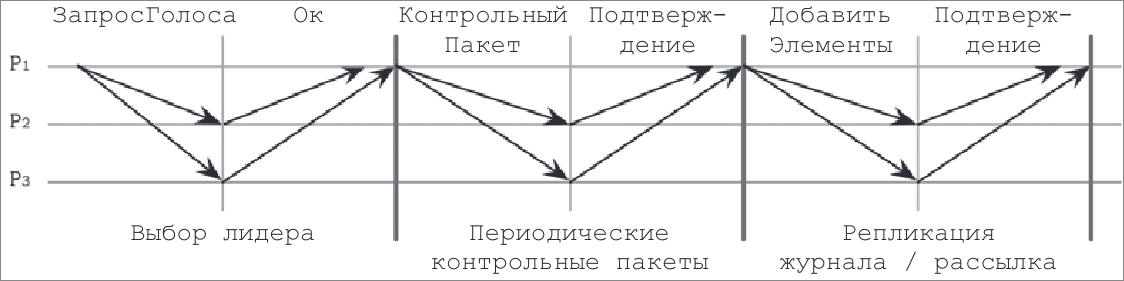
\includegraphics[scale=0.4]{inc/raft.png}
  \caption{Схема раунда Raft}
  \label{fig:raft}
\end{figure}

\begin{itemize}
    \item Выбор лидера. Когда узел-кандидат (P1 на рисунке) решает стать лидером,
        он рассылает остальным участникам сообщение $ЗапросГолоса$, содержащее свой
        период, последнюю известную ему информацию о периоде, а также идентификатор
        самой свежей записи в журнале, которую он видел. Если кандидат получает
        большинство голосов, он становится лидером на текущий период. При этом
        каждый узел может отдать голос лишь одному кандидату.
    \item Периодические контрольные пакеты. Для поддержания жизнеспособности
        системы лидер с определённой периодичностью отправляет контрольные
        пакеты всем последователям, тем самым подтверждая своё лидерство. Если
        последователь не получает такие пакеты в течение «тайм-аута выборов»,
        он предполагает сбой лидера и инициирует новый процесс голосования.
    \item Репликация. Лидер может неоднократно пополнять реплицируемый журнал,
        отправляя сообщение $ДобавитьЭлементы$, где указывает период лидера,
        индекс и период последней зафиксированной записи, а также одну или
        несколько новых записей для сохранения.
\end{itemize}

\subsection{Роль лидера в Raft}

Лидер может быть выбран только среди узлов, содержащих все актуальные записи.
Если в процессе выборов журнал последователя более актуальный, чем у кандидата,
то голос за этого кандидата не отдается.

Для победы в голосовании кандидат должен получить большинство голосов. Поскольку
записи реплицируются строго по порядку, достаточно сравнить идентификаторы последних
записей. После избрания лидер начинает принимать запросы от клиентов и реплицирует
их на своих последователей. Для этого он добавляет запись в свой журнал и
одновременно отправляет её всем последователям.

Когда последователь получает сообщение о добавлении записей, он вносит эти
записи в локальный журнал и отправляет подтверждение, сообщая лидеру, что данные
сохранены. Как только лидер получает достаточное количество подтверждений, запись
считается зафиксированной и помечается соответствующим образом в его журнале.

Поскольку лидером может стать только узел с наиболее актуальными данными,
последователь не отправляет ему обновления. Записи журнала передаются
только в одном направлении — от лидера к последователям.

\begin{figure}
  \centering
  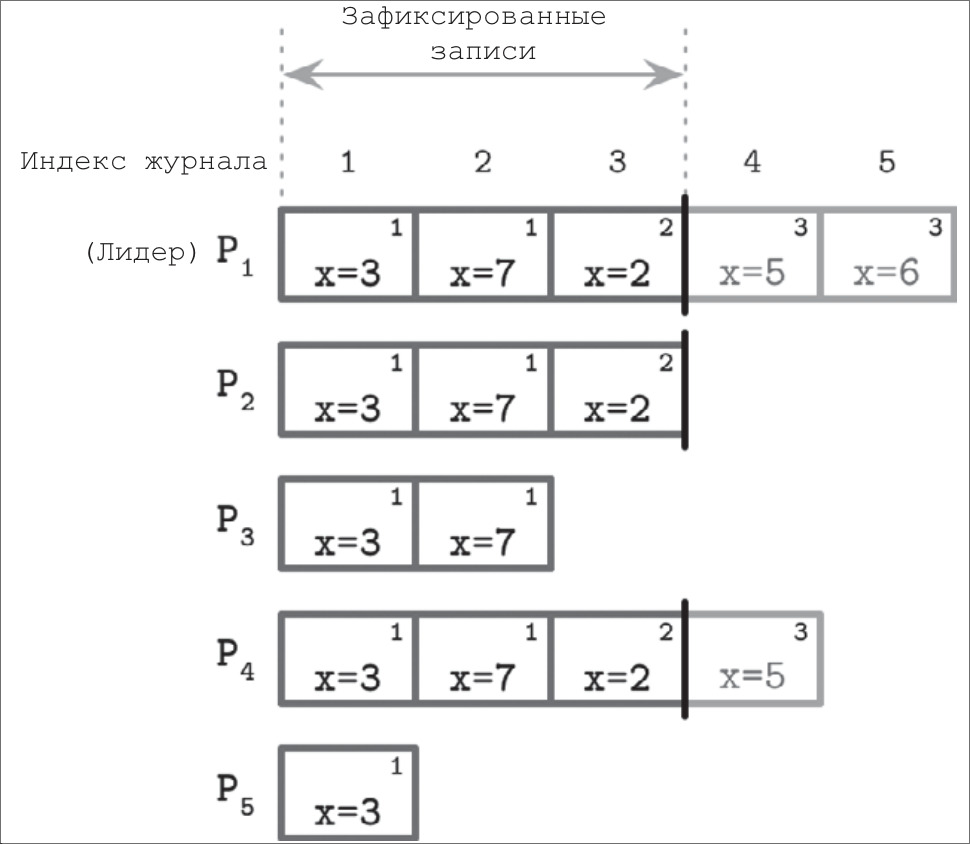
\includegraphics[scale=0.4]{inc/raft-consensus.png}
  \caption{Конечный автомат алгоритма Raft}
  \label{fig:raft-consensus}
\end{figure}

На рисунке \ref{fig:raft-consensus} представлен пример раунда достижения
консенсуса, в котором узел P1 выступает в роли лидера с наиболее актуальной
информацией. Лидер выполняет алгоритм, реплицируя записи на своих последователей
и фиксируя их после получения подтверждений. Фиксация одной записи автоматически
фиксирует все предшествующие записи в журнале. Решение о фиксации может принимать
только лидер. Каждая запись в журнале имеет идентификатор периода (терма, указан в
верхнем правом углу записи) и индекс, определяющий её позицию в журнале.
Зафиксированные записи гарантированно реплицируются на кворум узлов, что
позволяет безопасно применять их к конечному автомату в порядке их добавления.

\subsection{Сценарии отказов}

Когда несколько последователей решают стать кандидатами, но ни один из них не
может набрать большинство голосов, такая ситуация называется "разделенным
голосованием". Чтобы снизить вероятность таких случаев, алгоритм Raft применяет
рандомизированные таймеры. Это позволяет одному из кандидатов начать следующий
этап выборов раньше других, получить достаточное количество голосов и быть
избранным, пока остальные кандидаты находятся в ожидании. Такой подход ускоряет
процесс выборов, исключая необходимость дополнительной координации между кандидатами.

Если последователи отключаются или задерживают ответы, лидер обязан
предпринимать дополнительные попытки доставки сообщений. Если подтверждение от
узлов не поступает в ожидаемый срок, лидер повторно отправляет сообщения.

Благодаря уникальным идентификаторам, присваиваемым реплицируемым записям,
порядок в журнале остается неизменным, даже при повторной доставке сообщений.
Последователи устраняют дублирующие записи, основываясь на их порядковых номерах,
что предотвращает нежелательные эффекты от повторных отправок. Также порядковые
номера используются для соблюдения хронологии в журнале: последователь отклоняет
записи с более высокими номерами, если предыдущие записи не совпадают с
его журналом. Если две записи из разных журналов имеют одинаковые идентификаторы
и индексы, то они хранят одну и ту же команду, а все предшествующие им записи
идентичны.

Для обнаружения сбоев лидер отправляет последовательным узлам контрольные
сообщения, подтверждая тем самым активность своего периода. Если один из узлов
замечает, что текущий лидер перестал отвечать, он инициирует процедуру выборов.
Новый лидер восстанавливает состояние кластера, определяя последнюю согласованную
запись (то есть запись с наибольшим номером, которую разделяют лидер и последователь).
Он приказывает узлам удалить все незафиксированные записи после этой точки и
реплицирует актуальные записи из своего журнала. Лидер не удаляет и не
перезаписывает собственные записи, а только добавляет новые.

Таким образом, Raft предоставляет следующие гарантии:

\begin{itemize}
    \item Только один лидер может быть избран одновременно на заданный период (терм);
        в течение одного периода не может быть двух активных лидеров;
    \item Лидер не удаляет и не переупорядочивает содержимое журнала; он только
        добавляет новые сообщения к нему;
    \item Зафиксированные записи в журнале гарантированно присутствуют в журналах
        для последующих лидеров;
    \item Все сообщения однозначно идентифицируются по идентификаторам сообщений
        и периодов; ни текущий, ни последующие лидеры не могут повторно использовать
        один и тот же идентификатор для другой записи.
\end{itemize}

